% Generated by plot_tldr_results.py.
% Copy the snippets you need into the paper. Captions are intentionally outside the figures.

\begin{figure}[t]
    \centering
    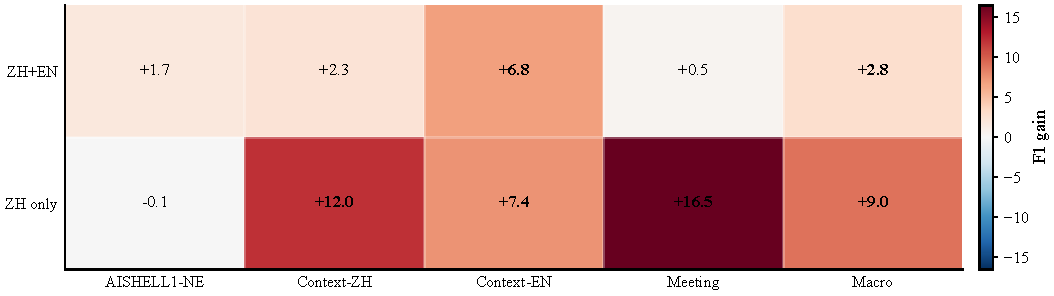
\includegraphics[width=\textwidth]{figures/fig1_tldr_gain_heatmap.pdf}
    \caption{Summary of TLDR's absolute F1 gain over the strongest baseline. The gain is small on saturated in-domain settings and grows under restricted or difficult conditions.}
    \label{fig:tldr-gain-heatmap}
\end{figure}

\begin{figure}[t]
    \centering
    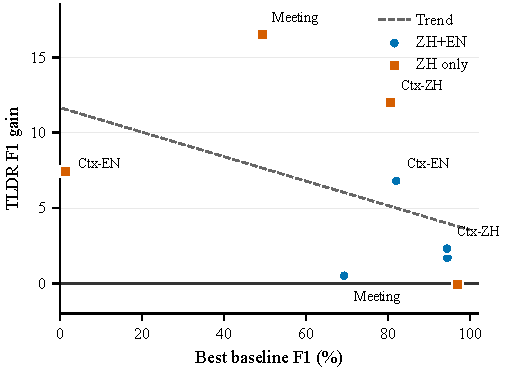
\includegraphics[width=0.48\textwidth]{figures/fig2_difficulty_vs_gain.pdf}
    \caption{Relationship between baseline difficulty and TLDR improvement. Each point is one training regime and test dataset; the dashed line is a least-squares guide.}
    \label{fig:difficulty-gain}
\end{figure}

\begin{figure}[t]
    \centering
    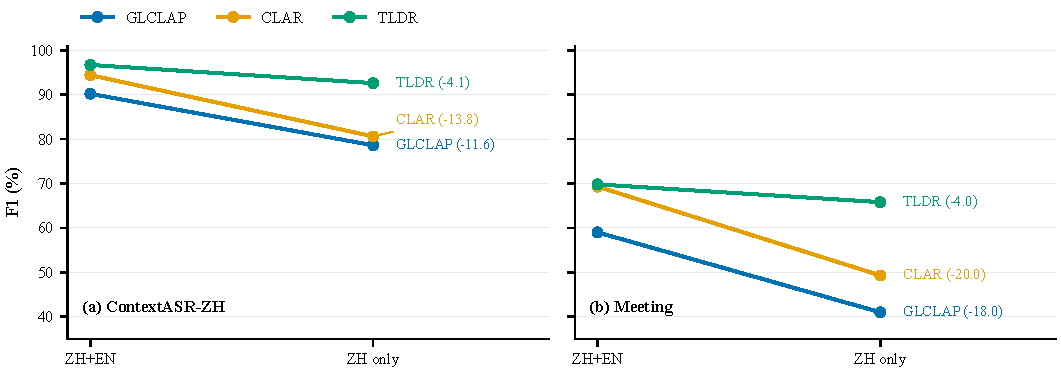
\includegraphics[width=\textwidth]{figures/fig3_restricted_training_degradation.pdf}
    \caption{F1 degradation from bilingual training to Chinese-only training on two cross-domain Chinese test sets. Values in parentheses denote the absolute change in F1.}
    \label{fig:restricted-training}
\end{figure}

\begin{figure}[t]
    \centering
    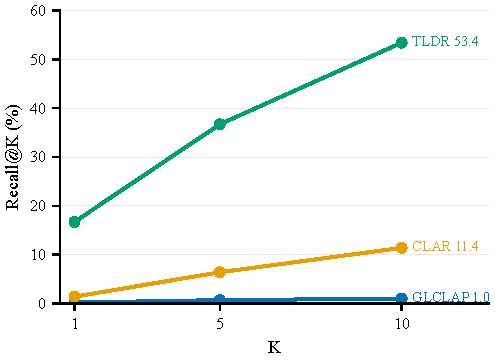
\includegraphics[width=0.48\textwidth]{figures/fig4_zh_only_contextasr_en_ranking.pdf}
    \caption{Zero-shot English candidate ranking under Chinese-only training. TLDR improves Recall@K substantially, while absolute detection performance remains limited.}
    \label{fig:zh-only-en-ranking}
\end{figure}

\begin{figure}[t]
    \centering
    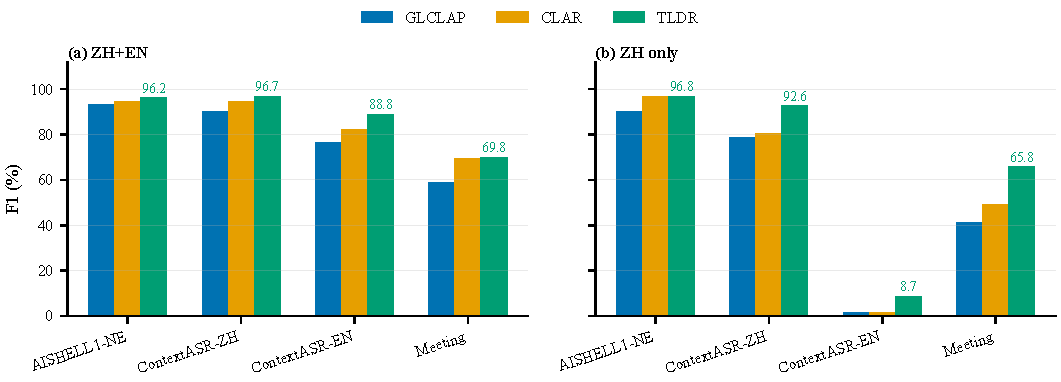
\includegraphics[width=\textwidth]{figures/figS1_detection_f1_overview.pdf}
    \caption{Complete F1 overview across datasets, training regimes, and models. TLDR bar values are annotated for readability.}
    \label{fig:f1-overview}
\end{figure}
